\documentclass{article}

\usepackage{amsmath}
\usepackage{fullpage}
\usepackage{url}
\usepackage{xspace}


\title{Examples of how to use functions}
\author{Kwame Okrah, Hector Bravo}
\date{\today}

\usepackage{Sweave}
\begin{document}
\Sconcordance{concordance:batch_vignette.tex:batch_vignette.Rnw:%
1 12 1 1 0 35 1 1 2 1 0 1 2 1 0 2 1 19 0 1 2 2 1 1 6 5 0 1 1 13 0 1 2 5 %
1 1 3 2 0 1 3 2 0 1 4 6 0 1 2 3 1 1 2 1 0 1 1 13 0 1 2 2 1 1 3 14 0 1 3 %
15 0 1 2 3 1 1 3 6 0 1 2 3 1 1 6 9 0 1 2 28 1 1 3 2 0 1 1 10 0 1 1 5 0 %
1 1 22 0 2 2 1 0 1 1 55 0 1 2 1 3 2 0 2 1 13 0 1 2 1 5 8 0 1 2 5 1 1 3 %
5 0 1 2 1 3 2 0 2 1 3 0 1 2 1 3 12 0 1 1 3 0 2 2 1 0 1 2 1 0 1 1 55 0 1 %
2 5 1}

\maketitle

\section{Overview of package}
The purpose of this package is to streamline the process for analyzing RNA-seq data
with potential batch effects. The pipeline includes 1) quantile normalization 2) log-transformation of counts 3) combat batch correction 4) voom calculation of weights for testing from mean-variance relationship.\\\\
The functions in this package can be grouped into two main categories:

\begin{enumerate}
\item The functions used for assessing batch effects.
    \begin{itemize}
    \item makeSVD
    \item pcRes
    \item plotPC
    \end{itemize}
\item The functions for removing batch effect and computing weights for limma.
    \begin{itemize}
    \item interpretZ
    \item qNorm
    \item log2CPM
    \item voomMod
    \item combatMod
    \item batchSEQ$^*$
    \end{itemize}
\end{enumerate}
$^*$ batchSEQ is the pipeline function. It combines qNorm, log2CPM, voomMod, and combatMod
into one step.\\\\
Below we will illustrte how to use these functions using the pasilla data set.\\\\
{\bf note}: All the functions in this package have a detailed help file which tells you
what kind of objects go in and what kind of objects come out. It is important to look
at these help files for each function.

\section{Examples of how to use the functions}
We will use the pasilla dataset found in the pasilla package. (This is the same dataset used
in the DESeq vignette)
\begin{Schunk}
\begin{Sinput}
> require(pasilla)
> # locate the path of the dataset and read in the dataset
> datafile <- system.file("extdata/pasilla_gene_counts.tsv", package="pasilla")
> counts <- read.table(datafile, header=TRUE, row.names=1)
> head(counts)
\end{Sinput}
\begin{Soutput}
            untreated1 untreated2 untreated3 untreated4 treated1 treated2
FBgn0000003          0          0          0          0        0        0
FBgn0000008         92        161         76         70      140       88
FBgn0000014          5          1          0          0        4        0
FBgn0000015          0          2          1          2        1        0
FBgn0000017       4664       8714       3564       3150     6205     3072
FBgn0000018        583        761        245        310      722      299
            treated3
FBgn0000003        1
FBgn0000008       70
FBgn0000014        0
FBgn0000015        0
FBgn0000017     3334
FBgn0000018      308
\end{Soutput}
\end{Schunk}
In this dataset there are two biological conditions treated (3 samples) and untreated (4 samples). 
Two samples are single-end and the other 4 are paired-end. We will use sigle-end and paired-end
as bathch effects. Below is the design (pheno data.frame).
\begin{Schunk}
\begin{Sinput}
> design <- data.frame(row.names=colnames(counts), 
+                     condition=c("untreated","untreated","untreated",
+                                 "untreated","treated","treated","treated"),
+                     libType=c("single-end","single-end","paired-end",
+                               "paired-end","single-end","paired-end","paired-end"))
> design
\end{Sinput}
\begin{Soutput}
           condition    libType
untreated1 untreated single-end
untreated2 untreated single-end
untreated3 untreated paired-end
untreated4 untreated paired-end
treated1     treated single-end
treated2     treated paired-end
treated3     treated paired-end
\end{Soutput}
\end{Schunk}
\subsection{Explore data for batch effects}
We will begin our analysis by exploring the data for possible/significant batch effects. We will 
begin by calling the function makeSVD on counts. This fucntion produces the pricipal components 
data necessary for any futher exploratory analysis. However, before calling makeSVD on the
counts we must normalize the counts. We will normalize the counts using the qauntile normalization 
method via the function qNorm.
\begin{Schunk}
\begin{Sinput}
> # load batch package
> require(batch)
> #
> # quantile normalize
> qcounts <- qNorm(counts)
> #
> # conpute princ. comp. data. 
> # returns a list with two components v and d.
> res <- makeSVD(qcounts)
\end{Sinput}
\end{Schunk}
We can now call pcRes and plotPC.
\begin{itemize}
\item pcRes: computes variance of each principal component and how they correlate with batch and condition.\\\\
Explain results in table: Hector
\begin{Schunk}
\begin{Sinput}
> tab <- pcRes(res$v,res$d, design$condition, design$libType)
> tab
\end{Sinput}
\begin{Soutput}
  propVar cumPropVar cond.R2 batch.R2
1   49.25      49.25   94.59     0.03
2   28.36      77.61    0.51    80.14
3   11.16      88.77    3.24    13.68
4    5.38      94.15    0.06     4.96
5    4.56      98.71    1.57     1.07
6    1.29     100.00    0.04     0.12
7    0.00     100.00    0.85     0.74
\end{Soutput}
\end{Schunk}
We can call pcRes without batch nor condition. This can be useful when a specific batch
is not known a priori. In our example we can pretend not to know that libType is a batch effect.\\\\
Explain results in table: Hector
\begin{Schunk}
\begin{Sinput}
> # call without batch
> pcRes(res$v,res$d, design$condition)
\end{Sinput}
\begin{Soutput}
  propVar cumPropVar cond.R2
1   49.25      49.25   94.59
2   28.36      77.61    0.51
3   11.16      88.77    3.24
4    5.38      94.15    0.06
5    4.56      98.71    1.57
6    1.29     100.00    0.04
7    0.00     100.00    0.85
\end{Soutput}
\begin{Sinput}
> #
> # call without batch nor condition
> pcRes(res$v,res$d)
\end{Sinput}
\begin{Soutput}
  propVar cumPropVar
1   49.25      49.25
2   28.36      77.61
3   11.16      88.77
4    5.38      94.15
5    4.56      98.71
6    1.29     100.00
7    0.00     100.00
\end{Soutput}
\end{Schunk}
\newpage
\item plotPC: Plot first 2 principal components. This function works like the regular plot function 
in R. ie. We can add all the options to make the plot sensible and well labelled. Below is an 
example:
\begin{Schunk}
\begin{Sinput}
> # a 'raw' plot the first 2 principal components
> plotPC(res$v, res$d)
\end{Sinput}
\end{Schunk}
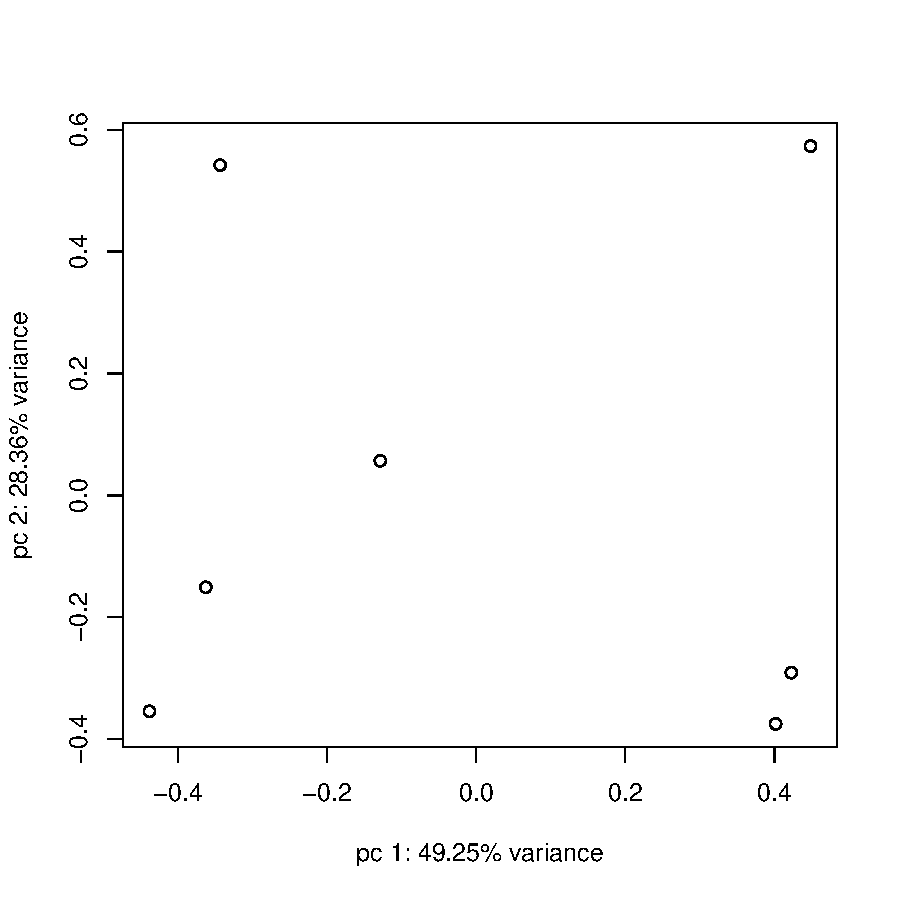
\includegraphics{batch_vignette-006}
As we can see this plot is not very useful since we have not labelled the points. We can choose
to labell the plot in anyway we see fit. In the example below we label batch with the shape of 
the point and condition with color.
\newpage
\begin{Schunk}
\begin{Sinput}
> # a labelled plotPC
> plotPC(res$v,res$d, 
+        col=design$condition, # color by batch
+        pch=ifelse(design$libType=="single-end", 21, 22), # shape be condition
+        main="Principal component plot: count scale")
\end{Sinput}
\end{Schunk}
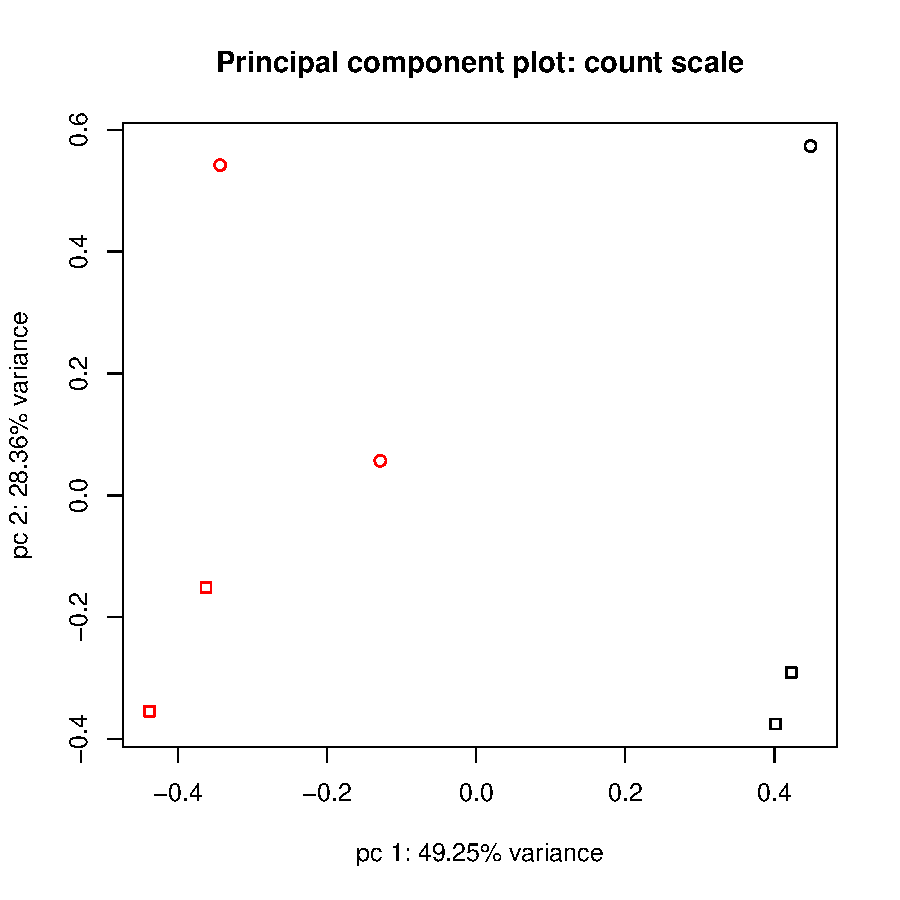
\includegraphics{batch_vignette-007}
\end{itemize}
We have shown how to use the three `exploratory' functions (makeSVD, pcRes, pcPlot). Note that 
we could have worked with log2(quantile counts per mil reads) instead.
% \newpage
% <<>>=
% # produces a list of log2(quantile counts per mil reads) and lib.size
% hold <- log2CPM(qcounts)
% names(hold) # look at names of result list
% res2 <- makeSVD(hold$y) # grab y component and make svd
% tab2 <- pcRes(res2$v,res2$d, design$condition, design$libType)
% tab2
% @
% 
% <<fig=TRUE>>=
% # a labelled plotPC
% plotPC(res2$v, res2$d, 
%        col=design$condition, # color by batch
%        pch=ifelse(design$libType=="single-end", 21, 22), # shape be condition
%        main="Principal component plot: log scale")
% @

\subsection{Correct data for batch effects}
To correct for the batch effect we call the pipeline function batchSEQ. In addition to 
counts(raw unadjusted counts), batch and condition; batchSEQ requires a model matrix.
More to come on model matrices later. batchSEQ produces a list with 2 components.
\begin{enumerate}
\item elist: a special list that limma will use. It contains the log counts, weights, model matrix, etc. (Consult limma vignette for details.)
\item combatEstimates: this is a list of dataframes containing the location (gamma star) and scale (delta.star) batch adjustments. 
\end{enumerate}
\begin{Schunk}
\begin{Sinput}
> # make model matrix
> mod <- model.matrix(~1+condition, data=design)
> res <- batchSEQ(counts, mod, design$libType, design$condition)
\end{Sinput}
\begin{Soutput}
Found 2 batches
Found 1  categorical covariate(s)
Standardizing Data across genes
Fitting L/S model and finding priors
Finding parametric adjustments
Adjusting the Data
\end{Soutput}
\begin{Sinput}
> names(res)
\end{Sinput}
\begin{Soutput}
[1] "elist"           "combatEstimates"
\end{Soutput}
\begin{Sinput}
> lapply(res$combatEstimates, head)
\end{Sinput}
\begin{Soutput}
$gamma.star
                  [,1]       [,2]
FBgn0000003  0.2928072 -0.3904103
FBgn0000008  0.9655716 -1.2874298
FBgn0000014 -1.2106506  1.6142024
FBgn0000015  0.3734137 -0.4978840
FBgn0000017  0.1147053 -0.1529403
FBgn0000018 -1.1245230  1.4993651

$delta.star
                 [,1]     [,2]
FBgn0000003 1.2914241 1.373908
FBgn0000008 1.3384449 1.322961
FBgn0000014 0.8133786 1.891870
FBgn0000015 0.9550527 1.738366
FBgn0000017 1.1363244 1.541959
FBgn0000018 0.9340701 1.761101
\end{Soutput}
\end{Schunk}
Now let us look at the elist component.
\begin{Schunk}
\begin{Sinput}
> edat <- res$elist
> edat
\end{Sinput}
\begin{Soutput}
An object of class "EList"
$E
            untreated1 untreated2 untreated3 untreated4  treated1  treated2
FBgn0000003  -4.543729  -4.543719  -4.862002  -4.861996 -4.462816 -4.795887
FBgn0000008   3.013946   3.066404   3.200762   2.848860  2.883463  3.107789
FBgn0000014  -2.759650  -4.952594  -3.739420  -3.739413 -3.590360 -3.753271
FBgn0000015  -4.031439  -2.638528  -2.951436  -2.177098 -3.914614 -5.013403
FBgn0000017   8.420187   8.619230   8.691529   8.398937  8.369435  8.325155
             treated3
FBgn0000003 -3.179835
FBgn0000008  2.705278
FBgn0000014 -3.753277
FBgn0000015 -5.013409
FBgn0000017  8.339088
14594 more rows ...

$weights
           [,1]       [,2]       [,3]       [,4]       [,5]       [,6]
[1,]   1.847105   1.847105   1.847105   1.847105   2.041169   2.041153
[2,]  35.608297  35.608084  35.607149  35.607022  33.127785  33.127140
[3,]   2.202885   2.202879   2.202855   2.202852   2.252523   2.252505
[4,]   2.692073   2.692066   2.692034   2.692029   1.847105   1.847105
[5,] 143.624879 143.624870 143.624834 143.624829 143.464818 143.464781
           [,7]
[1,]   2.041156
[2,]  33.127242
[3,]   2.252508
[4,]   1.847105
[5,] 143.464787
14594 more rows ...

$design
           (Intercept) conditionuntreated
untreated1           1                  1
untreated2           1                  1
untreated3           1                  1
untreated4           1                  1
treated1             1                  0
treated2             1                  0
treated3             1                  0
attr(,"assign")
[1] 0 1
attr(,"contrasts")
attr(,"contrasts")$condition
[1] "contr.treatment"


$lib.size
untreated1 untreated2 untreated3 untreated4   treated1   treated2   treated3 
  13238533   13238432   13237990   13237930   13238498   13238164   13238217 
\end{Soutput}
\end{Schunk}
At this point we can check our results to see have `removed' batch effects.
\begin{Schunk}
\begin{Sinput}
> # grab batch adjusted log counts from the elist
> res2 <- makeSVD(edat$E)
> tab2 <- pcRes(res2$v,res2$d, condition=design$condition, batch=design$libType)
> tab2
\end{Sinput}
\begin{Soutput}
  propVar cumPropVar cond.R2 batch.R2
1   36.50      36.50   94.74     2.54
2   21.00      57.50    1.42     0.05
3   17.38      74.88    0.04     0.00
4   15.18      90.06    1.37     0.09
5    9.94     100.00    2.43     0.12
6    0.00     100.00    0.00    97.19
7    0.00     100.00    0.00    97.19
\end{Soutput}
\end{Schunk}
\newpage
\begin{Schunk}
\begin{Sinput}
> plotPC(res2$v, res2$d, 
+        col=design$condition, # color by batch
+        pch=ifelse(design$libType=="single-end", 21, 22), # shape be condition
+        main="Principal component plot: log scale")
\end{Sinput}
\end{Schunk}
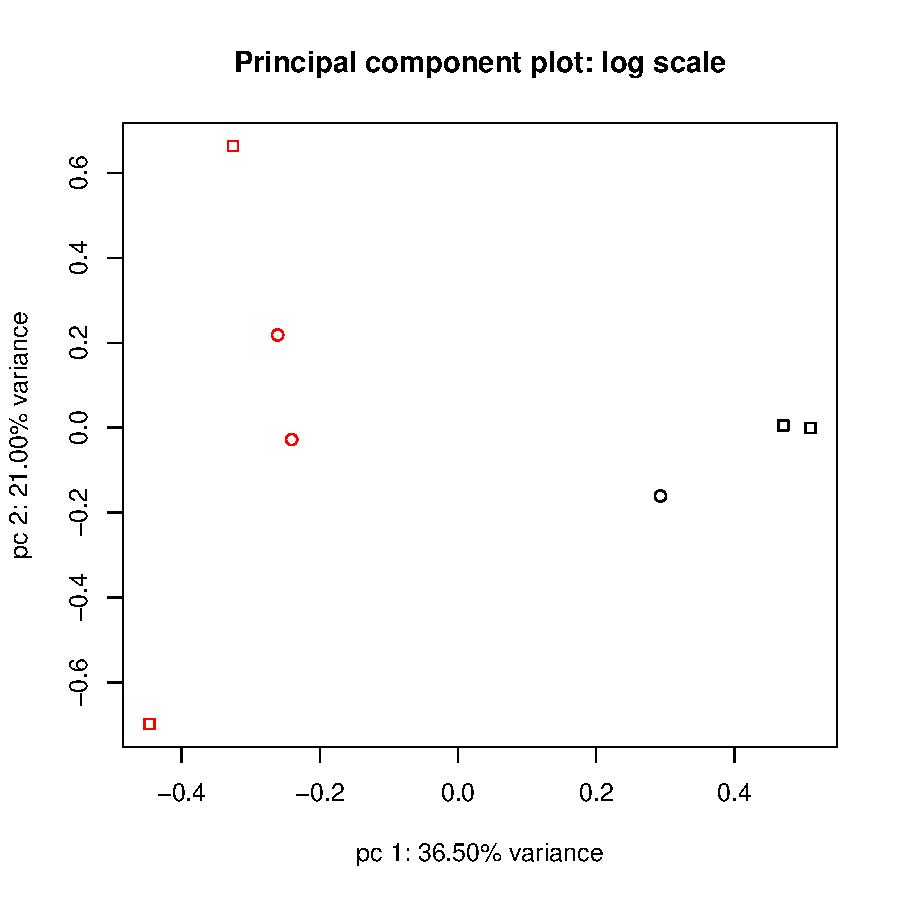
\includegraphics{batch_vignette-011}

The data is now ready for statistical analyis. Note that we could have achieved the results of the
batchSEQ function by calling the individual functions in the pipelie.

\begin{enumerate}
\item Quantile normalization.
\begin{Schunk}
\begin{Sinput}
> # see help for input and output
> qcounts <- qNorm(counts) 
\end{Sinput}
\end{Schunk}
\item Log-transform quantile normalized counts.
\begin{Schunk}
\begin{Sinput}
> # see help for input and output
> res <- log2CPM(qcounts) 
> y <- res$y
> lib.size <- res$lib.size
\end{Sinput}
\end{Schunk}
\item Combat batch correction
\begin{Schunk}
\begin{Sinput}
> # see help for input and output
> res <- combatMod(res$y, design$libType, design$condition)
\end{Sinput}
\begin{Soutput}
Found 2 batches
Found 1  categorical covariate(s)
Standardizing Data across genes
Fitting L/S model and finding priors
Finding parametric adjustments
Adjusting the Data
\end{Soutput}
\begin{Sinput}
> y <- res$bayesdata
\end{Sinput}
\end{Schunk}
\item Voom calculation of weights for testing from mean-variance relationship
\begin{Schunk}
\begin{Sinput}
> mod <- model.matrix(~1+condition, data=design)
> # see help for input and output
> voomRes <- voomMod(y, mod, lib.size, plot=FALSE)
> voomRes
\end{Sinput}
\begin{Soutput}
An object of class "EList"
$E
            untreated1 untreated2 untreated3 untreated4  treated1  treated2
FBgn0000003  -4.543729  -4.543719  -4.862002  -4.861996 -4.462816 -4.795887
FBgn0000008   3.013946   3.066404   3.200762   2.848860  2.883463  3.107789
FBgn0000014  -2.759650  -4.952594  -3.739420  -3.739413 -3.590360 -3.753271
FBgn0000015  -4.031439  -2.638528  -2.951436  -2.177098 -3.914614 -5.013403
FBgn0000017   8.420187   8.619230   8.691529   8.398937  8.369435  8.325155
             treated3
FBgn0000003 -3.179835
FBgn0000008  2.705278
FBgn0000014 -3.753277
FBgn0000015 -5.013409
FBgn0000017  8.339088
14594 more rows ...

$weights
           [,1]       [,2]       [,3]       [,4]       [,5]       [,6]
[1,]   1.847105   1.847105   1.847105   1.847105   2.041169   2.041153
[2,]  35.608297  35.608084  35.607149  35.607022  33.127785  33.127140
[3,]   2.202885   2.202879   2.202855   2.202852   2.252523   2.252505
[4,]   2.692073   2.692066   2.692034   2.692029   1.847105   1.847105
[5,] 143.624879 143.624870 143.624834 143.624829 143.464818 143.464781
           [,7]
[1,]   2.041156
[2,]  33.127242
[3,]   2.252508
[4,]   1.847105
[5,] 143.464787
14594 more rows ...

$design
           (Intercept) conditionuntreated
untreated1           1                  1
untreated2           1                  1
untreated3           1                  1
untreated4           1                  1
treated1             1                  0
treated2             1                  0
treated3             1                  0
attr(,"assign")
[1] 0 1
attr(,"contrasts")
attr(,"contrasts")$condition
[1] "contr.treatment"


$lib.size
untreated1 untreated2 untreated3 untreated4   treated1   treated2   treated3 
  13238533   13238432   13237990   13237930   13238498   13238164   13238217 
\end{Soutput}
\end{Schunk}
\end{enumerate}

\section{Design Matrix and Statistical Analysis via Limma}

More on this after we meet.
\end{document}
